\documentclass{beamer}

\usepackage{graphicx}

\title{Thumbs Up?  \\ Learning to Classify Useful Reviews}
\author{Ertan Dogrultan \and Cesar Romero \and Paul Wais\\
% Computer Science Department \\
% University of California, Los Angeles\\
% Los Angeles, California 90095\\
\texttt{\{ertan,romero,pwais\}@cs.ucla.edu}}
\date{November 29, 2010}
\begin{document}
\maketitle{}

\begin{frame}{User Votes Inform Review Sorting and Search}
\begin{figure}[h]
  \centering
  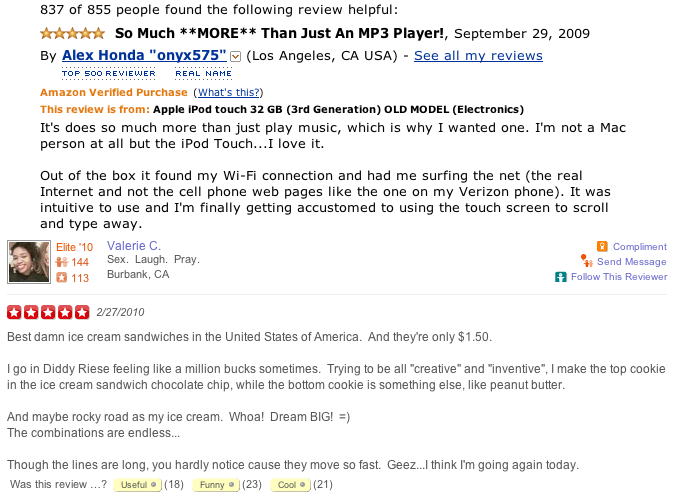
\includegraphics[scale=.4]{review_ex_1}
  \label{fig:dist}
\end{figure}
\end{frame}

\begin{frame}{Unfortunately, votes are sparse ...}
\begin{figure}[h]
  \centering
  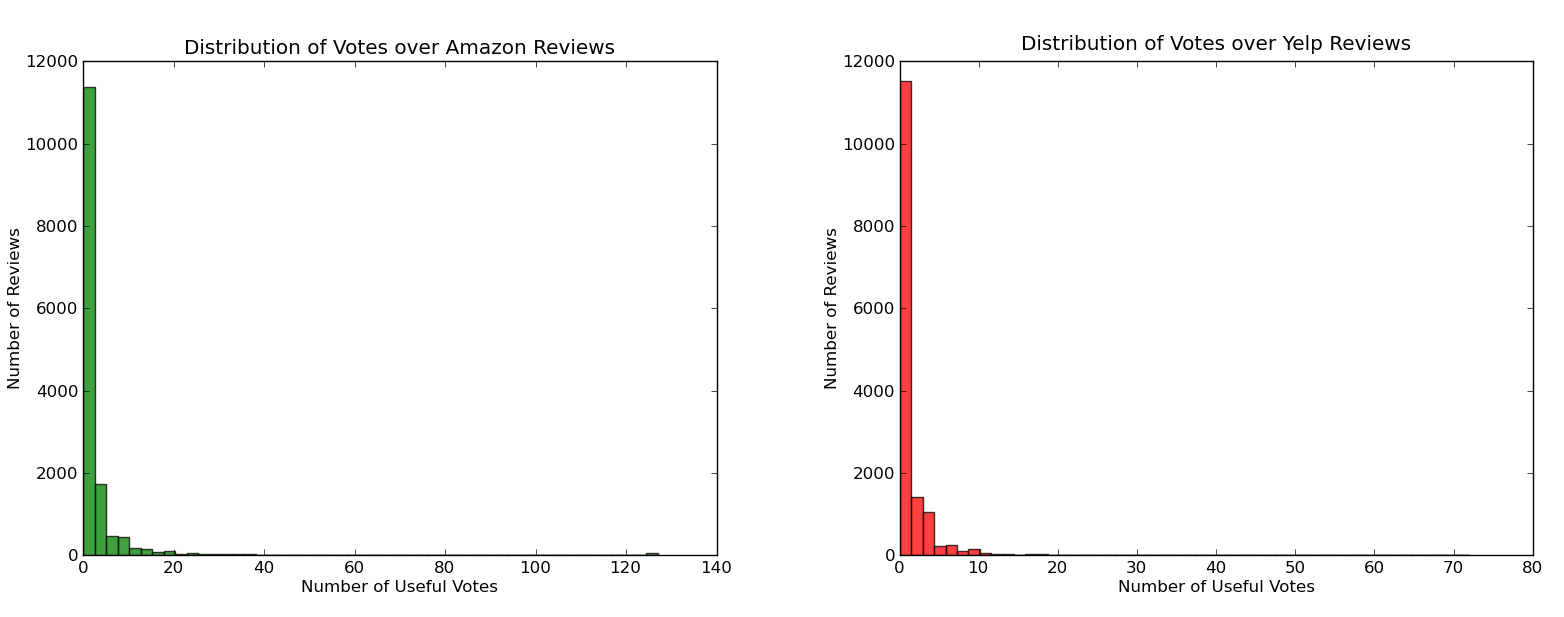
\includegraphics[width=\linewidth]{histos}
  \label{fig:dist}
\end{figure}
\end{frame}

\begin{frame}{... and there are many useful (and not so useful) reviews without votes}
\begin{figure}[h]
  \centering
  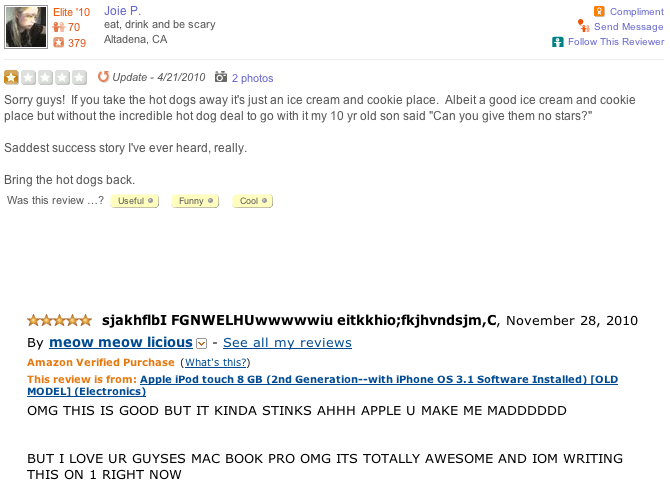
\includegraphics[scale=.4]{review_unvoted}
  \label{fig:dist}
\end{figure}
\end{frame}

\begin{frame}{Usefulness is Independent of Sentiment}
\begin{figure}[h]
  \centering
  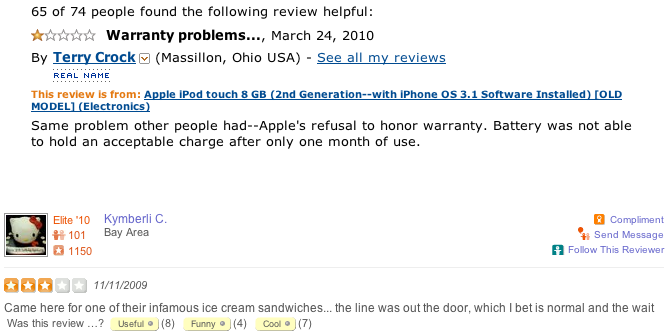
\includegraphics[scale=.4]{review_ex_2}
  \label{fig:dist}
\end{figure}
\end{frame}


\begin{frame}{Goal: Automatically Classify Reviews as (Un)Useful}
\begin{figure}[h]
  \centering
  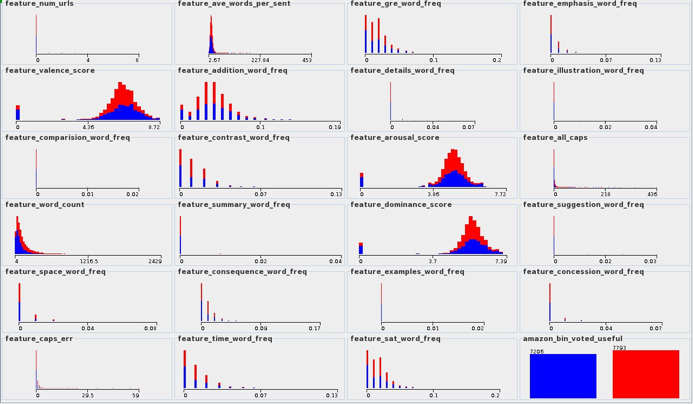
\includegraphics[scale=.4]{features_distributions}
  \caption{The distributions of the features}
  \label{fig:dist}
\end{figure}
\end{frame}

\begin{frame}{Features for Classifying Reviews}
\begin{figure}[h]
  \centering
  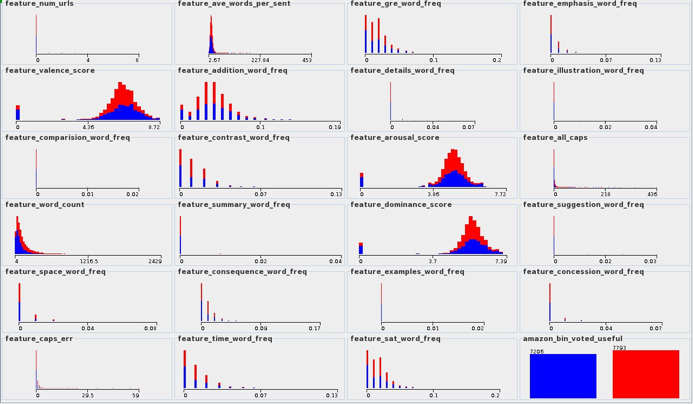
\includegraphics[scale=.4]{features_distributions}
  \caption{The distributions of the features}
  \label{fig:dist}
\end{figure}
\end{frame}

\begin{frame}{Feature Distributions}
\begin{figure}[h]
  \centering
  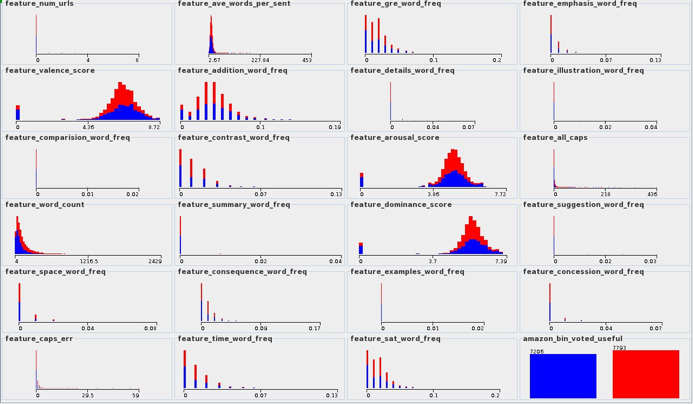
\includegraphics[scale=.4]{features_distributions}
  \caption{The distributions of the features}
  \label{fig:dist}
\end{figure}
\end{frame}

\begin{frame}{Cross-validation accuracy of the algorithms}
\begin{table}[ht]
  \centering
  \begin{tabular}{c | c}
    Algorithm    & Accuracy \\
    \hline
    SVM (RBF)    & 70.13\%  \\
    SVM (Linear) & 75\%     \\
    Adaboost     & 80\%     \\
    Naive Bayes  & 68.5\%   \\
    Winnow       & 56\%     \\
  \end{tabular}
  \caption{The 10 fold cross-validation accuracy of the algorithms}
  \label{tab:performance}
\end{table}
\end{frame}

\begin{frame}{Complications}
Why do different algorithms perform differently on this task?
\begin{itemize}
\item SVM
\item Adaboost
\item Naive Bayes 
\end{itemize}
\end{frame}

\begin{frame}{Future Work}
\begin{itemize}
\item Domain adaptation experiments
\begin{figure}[ht]
\centering
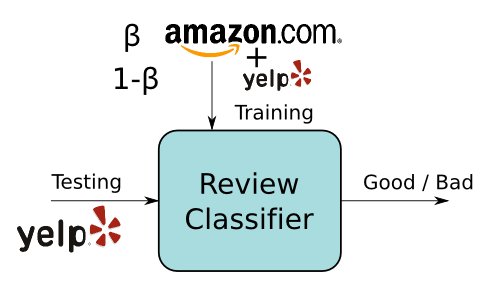
\includegraphics[scale=.3]{adaptation}
\label{fig:adaptation}
\end{figure}
\item Connections with the theoretical bounds
\end{itemize}

\end{frame}
\end{document}
